\section{SIMULAÇÃO} 

Segundo \citeonline{Garcia2009b} simulação é:

\begin{citacao}
A obtenção da resposta temporal das variáveis de interesse (variáveis dependentes) de um modelo, quando se excita suas variáveis de entrada com sinais desejados e se definem os valores das condições iniciais das variáveis dependentes.
\end{citacao}

A Figura \ref{simulacao} representa um modelo simplificado de um processo passível de simulação, onde $X$ é conjunto de variáveis de entrada, $Y$ é o conjunto de variáveis de saída e $P$ são os parâmetros do sistema incluindo condições de contorno. 
Com base neste modelo, \citeonline{Garcia2009b} afirma que é possível simular as seguintes aplicações:
\begin{enumerate}
	\item Projeto de equipamentos, processos e plantas e seus respectivos sistemas de controle;
	\item Pré-operação e operação de plantas;
	\item Sistema de controle de processos;
	\item Otimização das condições operacionais de plantas.
\end{enumerate}


\begin{figure}[ht]
	\centering
	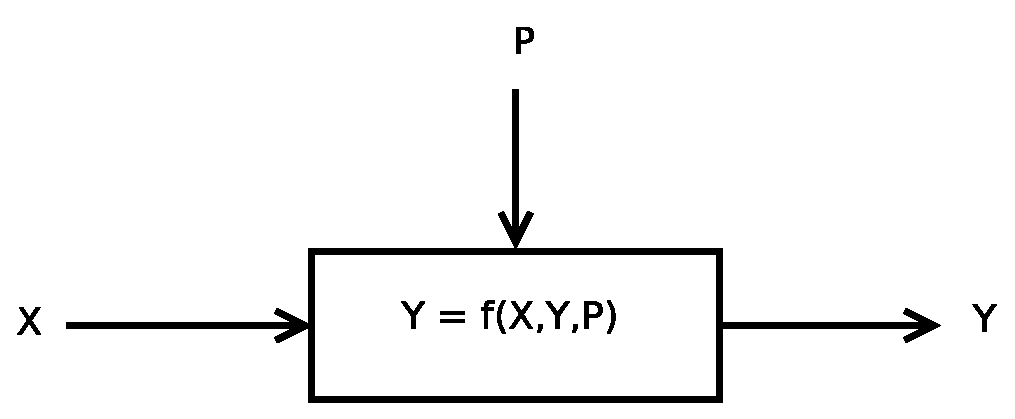
\includegraphics[width=10 cm]{figuras/simulacao.eps}
	\caption{Modelo matemático simplificado de um processo. Fonte: \citeonline{Garcia2009b}.}
    	\label{simulacao}
\end{figure}
